\chapter{Introduction}
\label{chapter:introduction}

%%% SECTION

\section{Motivation}

%%%%%%%%%%%%%%%%%%%
%%% Motivation %%%
%%%%%%%%%%%%%%%%%%%
This journey towards the realization of this exciting work on dermoscopic classification of skin disease is a path that combines science, technology and medical care in a unique way. This project is much more than a task at the end of a long master's journey; it is a challenge and an opportunity.

This job represents a challenge, working with large image files which require pre-processing of data. Added to this is the development of a classification model that must distinguish between nine different patterns. All these points are compounded by the fact of doing the work in a language that is not my mother tongue.

On the other hand, it also represents an opportunity to imagine that my work could one day help in the early detection of skin disease, and thus improve medical care.


\section{Goals}

%%%%%%%%%%%%%%%%%%%
%%% Goals %%%
%%%%%%%%%%%%%%%%%%%

The main objective of this project is the classification of dermoscopic images. This challenge can be separated into two points

\begin{itemize}
    \item On the one hand, to distinguish dermatological skin lesions.
    \item Secondly, to classify these lesions into one of nine classes to be studied.
\end{itemize}

In parallel, the dataset contains a metadata file. This information can help to segment the source information according to the types of dermoscopic techniques used. Therefore, this provides us with a secondary objective by allowing us to make a reliability ranking according to the technique used. 


\section{Methodology}

%%%%%%%%%%%%%%%%%%%
%%% Methodology %%%
%%%%%%%%%%%%%%%%%%%

\section{Planning}

%%%%%%%%%%%%%%%%%%%
%%% Planning %%%
%%%%%%%%%%%%%%%%%%%
The project has been structured in five phases or modules, which in turn are broken down into tasks. This section describes the project's planning and its main milestones. 
\begin{itemize}
    \item \textbf{Module 1 - Project definition} 
    
    This module starts with the definition of the project plan: the relevant objectives of the project, the initial planning that will form the basis of the project, and the personal motivation to carry out the project on the chosen topic. During this phase, the abstract of the work will also be written and the "Ethical and personal data protection protocol" will be presented.
    \item \textbf{Module 2 - State of Art}
    
    During the time of this module, we will carry out a research phase in which we will search for previous or current scientific work related to the main topic of this project.
    \item \textbf{Module 3 - Design \& implementation}
    
    The objectives of this activity are to carry out the tasks necessary for the design and development of the project according to the chosen scientific methodology. During this period, the progress made will be documented in order to complement the project document. 
    \item \textbf{Module 4 - Document redaction}
    
    The purpose of this activity is to prepare all the materials required for the presentation and final assessment of the TFM (Master's Thesis). These materials include:
    
    \begin{enumerate}
        \item The Master's Thesis document
        \item An audiovisual presentation
    \end{enumerate}

    \item \textbf{Module 5 - Project defence}
    
    Finally, the final step of the Master's Thesis is to defend it before a board of examiners.
\end{itemize}

The following table shows each of the phases, the start and end dates, as well as the estimated effort.


\begin{table}[H]
    \resizebox{\textwidth}{!}{%
    \begin{tabular}{@{}clcccc@{}}
        \toprule
        \textbf{Module}            & \textbf{Description}     & \textbf{Start Date}     & \textbf{End Date}     & \textbf{days} 
   & \textbf{Effort (h)} \\ \midrule
        \textbf{} 1 & Project definition & 09/27/23 & 10/10/23 & 13 & 26 \\
        \textbf{} 2 & State of Art & 10/11/23 & 10/24/23 & 13 & 26 \\
        \textbf{} 3 & Design \& Implementation & 10/25/23 & 12/19/23 & 55  & 110 \\
        \textbf{} 4 & Document redaction & 12/20/23 & 01/16/24 & 27  & 54 \\
        \textbf{} 5 & Project defence & 01/17/24 & 02/03/24 &  17 & 34 \\
        \bottomrule
    \end{tabular}%
    }
\end{table}



The following Gantt graph shows the project's evolution.

\begin{figure}[h]
    \begin{center}
        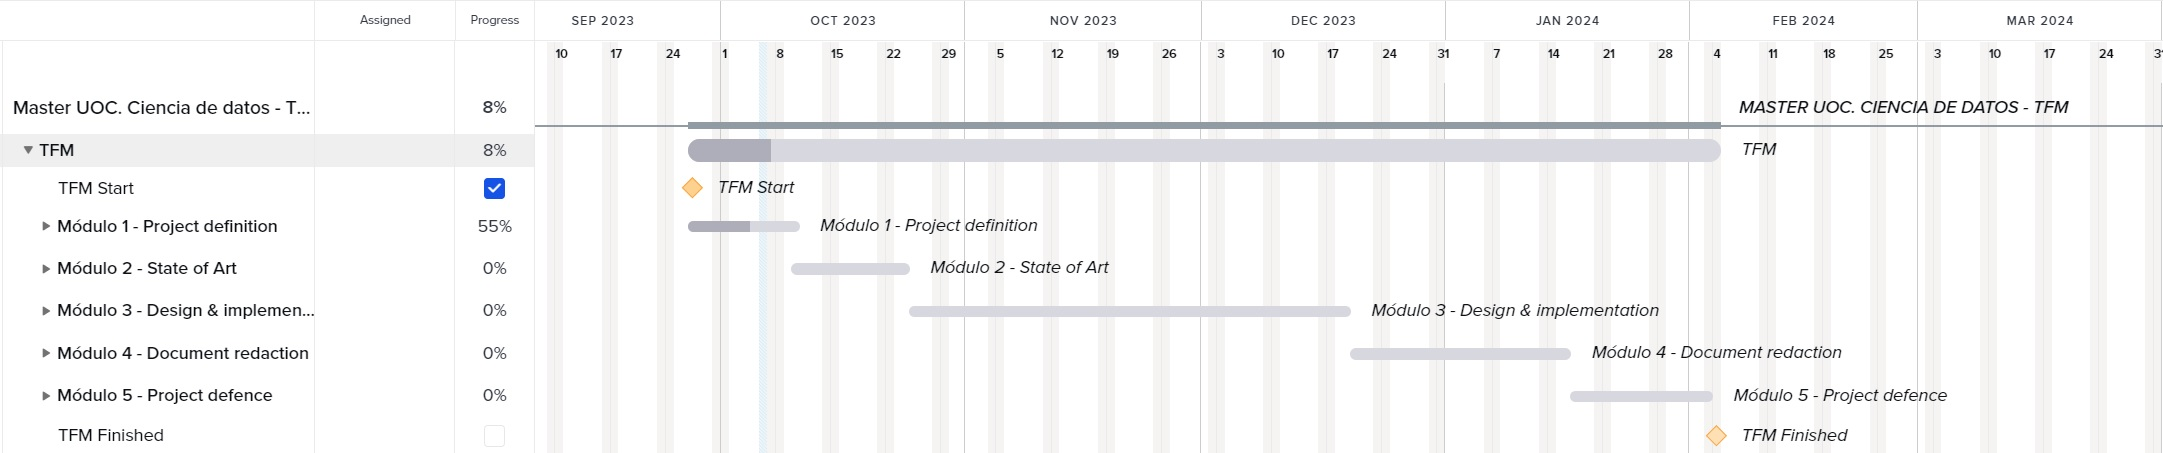
\includegraphics[scale=0.40]{images/TFM_Planing.jpg}
        \caption{Gantt chart of the Master's final project}
    \label{fig:Gantt}    
    \end{center}
\end{figure}